% Informe del proyecto final de Machine Learning (fuga de clientes, COFINFAD): datos, metodología y resultados del
% modelo original BDL. Compilar: python compilar.py   (usa Tectonic; ver README.md de esta carpeta)
\documentclass[11pt,a4paper]{article}

\usepackage[T1]{fontenc}
\usepackage[utf8]{inputenc}
\usepackage{lmodern}
\usepackage[spanish,es-tabla,es-noshorthands]{babel}
\usepackage[a4paper,textwidth=6.3in,textheight=9.4in,headheight=14pt]{geometry}
\usepackage{amsmath,amssymb,bm}
\usepackage{graphicx}
\usepackage{booktabs}
\usepackage{array}
\usepackage{caption}
\usepackage{algorithm}
\usepackage{algpseudocode}
\usepackage[authoryear,round]{natbib}
\usepackage{microtype}
\usepackage{xcolor}
\usepackage[section]{placeins}
\usepackage{xurl}
\usepackage[colorlinks=true,linkcolor=blue!55!black,citecolor=blue!55!black,urlcolor=blue!55!black]{hyperref}

\graphicspath{{figures/}}
\captionsetup{font=small,labelfont=bf,width=0.95\linewidth}
\renewcommand{\topfraction}{0.95}
\renewcommand{\bottomfraction}{0.6}
\renewcommand{\textfraction}{0.05}
\renewcommand{\floatpagefraction}{0.7}
\widowpenalty=10000 \clubpenalty=10000
\setlength{\parskip}{3pt plus 1pt}
\setlength{\bibsep}{3pt plus 1pt}
\floatname{algorithm}{Algoritmo}
\renewcommand{\algorithmicrequire}{\textbf{Entrada:}}
\renewcommand{\algorithmicensure}{\textbf{Salida:}}
\algrenewcommand\algorithmicfor{\textbf{para}}
\algrenewcommand\algorithmicdo{\textbf{hacer}}
\algrenewcommand\algorithmicend{\textbf{fin}}
\algrenewcommand\algorithmicif{\textbf{si}}
\algrenewcommand\algorithmicthen{\textbf{entonces}}

% Notación
\newcommand{\R}{\mathbb{R}}
\newcommand{\cp}{\texttt{churn\_\allowbreak probability}}
\newcommand{\ap}{\texttt{active\_\allowbreak products}}
\newcommand{\rmse}{\mathrm{RMSE}}

\title{\textbf{Predicción de la fuga de clientes de una \emph{fintech} con un boosting con desplazamiento latente (BDL):
datos, metodología y resultados}}
\author{Valerie Martínez Pulido, Abrahan Basto Martínez y Rubén Esguerra Fernández\\[4pt]
\small Proyecto final de Machine Learning\\ \small Pregrado en Ciencia de Datos, Universidad del Norte}
\date{Noviembre de 2026}

\begin{document}
\maketitle

% Introducción del informe del proyecto final (modelo original BDL).
\section{Introducción}\label{sec:introduccion}

Retener a un cliente cuesta menos que conseguir uno nuevo, y por eso una \emph{fintech} necesita ordenar a sus clientes
por riesgo de abandono antes de lanzar una campaña de retención de capacidad limitada. Este trabajo aborda ese problema
con COFINFAD \citep{munoz2025}, un conjunto público y sintético de $48.723$ clientes de una \emph{fintech} colombiana con
el detalle de sus transacciones de 2023, cuyo objetivo es un puntaje continuo de propensión al abandono, \cp.

En la versión anterior del proyecto, el modelo propuesto era una \emph{Explainable Boosting Machine} usada desde una
librería. Esta versión la reemplaza por un modelo propio, BDL (\emph{Boosting} con Desplazamiento Latente), que parte de
un hallazgo del análisis exploratorio: el puntaje es un índice suave de los predictores más un escalón constante que
depende de una variable que hay que excluir por fuga de información. BDL modela ese escalón como una clase latente y
aprende el índice con una regla de aprendizaje propia, un EM generalizado cuyo paso M es un paso de \emph{boosting}.

Las contribuciones son tres:
\begin{itemize}
  \item un modelo y su regla de aprendizaje, formulados, derivados y programados desde cero con \texttt{numpy} y
        \texttt{scipy}, con garantías teóricas verificadas por pruebas unitarias (sección~\ref{sec:modelo});
  \item una comparación con todos los modelos del curso y dos del estado del arte, bajo un protocolo registrado antes
        de los experimentos, con las mismas particiones, el mismo preprocesamiento y el mismo presupuesto de ajuste
        (secciones~\ref{sec:referencias} y~\ref{sec:protocolo});
  \item una evaluación estadística con tres pruebas de hipótesis por referencia, tamaños de efecto, cinco conjuntos de
        datos, ablación, sensibilidad, costo e interpretabilidad (sección~\ref{sec:resultados}).
\end{itemize}

La sección~\ref{sec:metodologia} describe los datos y su análisis exploratorio, el pipeline, los modelos de referencia,
el modelo propuesto y el protocolo de evaluación; la sección~\ref{sec:resultados} presenta los resultados, y la
sección~\ref{sec:conclusiones}, las conclusiones.

% Metodología del informe del proyecto final (modelo original BDL). Cifras del libro del proyecto y de
% ModeloOriginal/resultados; la tabla de hiperparámetros y la figura del pipeline las escribe generar.py.
\section{Metodología}\label{sec:metodologia}

Esta sección describe el problema, los datos y su análisis exploratorio, el pipeline, los modelos de referencia, el
modelo propuesto y el protocolo de evaluación; las cifras de desempeño se reservan para la sección~\ref{sec:resultados}.

\subsection{Formulación del problema y notación}\label{sec:formulacion}

Cada cliente $i$ se describe con un vector $\bm{x}_i \in \R^{p}$ ($p = 78$ columnas tras el preprocesamiento) y un
puntaje de propensión $s_i \in [0{,}114;\ 0{,}501]$, la columna \cp, que nunca vale 0 ni 1: es un puntaje, no un evento
observado. La tarea principal es la \textbf{regresión}: buscar $f: \R^p \to \R$ que minimice el error cuadrático medio,
\begin{equation}
  \mathcal{L}_R = \frac{1}{n}\sum_{i=1}^{n} (s_i - \hat{s}_i)^2, \qquad \rmse = \sqrt{\mathcal{L}_R},
  \label{eq:perdida}
\end{equation}
con el RMSE como métrica principal. La tarea secundaria es la \textbf{clasificación} del riesgo alto,
$y_i = \mathbf{1}[\,s_i > \tau\,]$, con $\tau$ el percentil 75 del puntaje estimado solo en el entrenamiento
($\tau = 0{,}3927$; $24{,}6$~\% de positivos), y el AUC como métrica. La Tabla~\ref{tab:notacion} resume la notación.

\begin{table}[htbp]
  \centering\small
  \caption{Notación principal.}
  \label{tab:notacion}
  \begin{tabular}{@{}>{\raggedright\arraybackslash}p{0.2\linewidth} >{\raggedright\arraybackslash}p{0.74\linewidth}@{}}
    \toprule
    Símbolo & Significado \\
    \midrule
    $\bm{x}_i \in \R^{p}$ & predictores del cliente $i$ tras el preprocesamiento ($p = 78$) \\
    $s_i$, $\hat{s}_i$ & puntaje \cp\ y su predicción \\
    $\tau$, $y_i$ & umbral de riesgo alto (percentil 75 del entrenamiento) y etiqueta $\mathbf{1}[s_i > \tau]$ \\
    $n$, $n_{\mathrm{te}}$ & clientes de entrenamiento ($38.978$) y de prueba ($9.745$) \\
    $F(\bm{x})$ & índice de BDL: una suma de árboles de regresión \\
    $z_i$, $K$ & clase latente del cliente (no se observa) y número de clases \\
    $\pi_k$, $c_k$, $\sigma$ & peso y desplazamiento de la clase $k$, y dispersión del error dentro de cada clase \\
    $\gamma_{ik}$ & probabilidad posterior de que el cliente $i$ pertenezca a la clase $k$ (paso E) \\
    $\tilde{s}_i$ & objetivo sin escalón: $s_i - \sum_k \gamma_{ik} c_k$ \\
    $\nu$, $d$, $M$, $\lambda$ & tasa de aprendizaje, profundidad de los árboles, intervalos por variable y penalización L2 de las hojas \\
    \bottomrule
  \end{tabular}
\end{table}

\subsection{Datos y análisis exploratorio}\label{sec:datos}

\paragraph{Fuente y tamaño.}
COFINFAD, \emph{Colombian Fintech Financial Analytics Dataset} \citep{munoz2025}, está publicado en Mendeley Data (DOI
10.17632/mhb4zn3258.1, licencia CC~BY~4.0). Describe a los clientes de una \emph{fintech} colombiana durante 2023 en dos
tablas: una con un registro por cliente ($48.723$ filas y $54$ columnas: perfil, tenencia de productos, uso digital,
satisfacción, resúmenes transaccionales y los objetivos) y otra con el detalle de $3.159.157$ transacciones. Los datos
son \textbf{sintéticos}: las conclusiones describen las reglas con que se generaron, no a clientes reales.

\paragraph{ETL.}
La auditoría del detalle no encontró montos no positivos, fechas nulas ni transacciones huérfanas, y eliminó $102$
transacciones duplicadas. Del detalle se derivaron doce variables de comportamiento por cliente (número de
transacciones; monto total, medio y mediano; recencia; días y meses activos; volatilidad del monto y proporción de cada
tipo de transacción), ninguna de las cuales usa el objetivo. Se eliminaron $17$ columnas con la evidencia de la
Tabla~\ref{tab:etl}. El único faltante que se conserva, \texttt{credit\_utilization\_ratio} ($37{,}4$~\% de los clientes
de entrenamiento), falta exactamente cuando el cliente no tiene tarjeta de crédito: es un \emph{no aplica} y se imputa
con cero. El conjunto final tiene $48$ predictores ($32$ numéricos, $9$ categóricos y $7$ booleanos), que el
preprocesamiento convierte en $p = 78$ columnas.

\begin{table}[tbp]
  \centering\small
  \caption{Columnas eliminadas en el ETL y razón de cada decisión (evidencia calculada solo con el entrenamiento).}
  \label{tab:etl}
  \begin{tabular}{@{}>{\raggedright\arraybackslash}p{0.34\linewidth} >{\raggedright\arraybackslash}p{0.6\linewidth}@{}}
    \toprule
    Columnas & Razón \\
    \midrule
    identificador del cliente & sin valor predictivo \\
    \ap & fuga de información: el puntaje se construyó a partir de ella (Figura~\ref{fig:objetivo}) \\
    valor del cliente y su segmento & son un segundo objetivo \\
    cuatro resúmenes transaccionales & duplican a otras columnas (dos con $r = 1{,}000$ con la frecuencia de transacciones) \\
    dos fechas & duplican a otras fechas \\
    tres fechas (\texttt{last\_survey\_date}, \texttt{first\_tx}, \texttt{last\_tx}) & sin señal ($\eta^2 = 0{,}0087$, $0{,}0046$ y $0{,}0044$) \\
    \texttt{nps\_score} & colineal con la satisfacción ($r = 0{,}917$) \\
    \texttt{occupation} & $35$ niveles sin señal ($\eta^2 = 0{,}0010$) \\
    dos columnas de texto & $50$~\% y $33$~\% de valores ausentes, sin mecanismo ni señal \\
    \bottomrule
  \end{tabular}
\end{table}

\paragraph{Hallazgos del análisis exploratorio.}
El puntaje tiene una distribución unimodal y asimétrica a la izquierda (asimetría $-0{,}61$; Figura~\ref{fig:objetivo},
izquierda), sin atípicos que tratar. Tres hallazgos condicionan el modelado. Primero, la edad solo toma seis valores
($29$, $30$, $44$, $45$, $59$ y $60$ años) agrupados en tres cohortes, en las que la proporción de riesgo alto va del
$8{,}7$ al $45{,}2$~\% sin crecer con la edad: una relación que un coeficiente lineal no representa y un árbol sí.
Segundo, \ap\ es la variable más asociada con el puntaje ($r = -0{,}876$; explica el $76{,}8$~\% de su varianza) y su
media desciende en escalones casi idénticos ($-0{,}0498$, $-0{,}0496$, $-0{,}0508$ y $-0{,}0496$; Figura~\ref{fig:objetivo},
derecha), con la misma dispersión ($0{,}032$) en cada nivel. Un paso constante es la firma de una regla de generación:
la variable se excluye por fuga de información \citep{kaufman2012}, y su escalón queda en el puntaje como un ruido de
cinco niveles que ningún predictor explica (al intentar predecirla con los demás, el AUC es $0{,}50$). Ese hallazgo
motiva el modelo propuesto. Tercero, sin ella la señal se concentra en pocas variables: correlaciones de Spearman de
$-0{,}279$ (frecuencia de uso de la aplicación), $+0{,}210$ (edad), $-0{,}190$ (satisfacción) y $-0{,}164$
(satisfacción de base), mientras que las doce variables transaccionales no aportan ($|\rho| \leq 0{,}018$).

\begin{figure}[tbp]
  \centering
  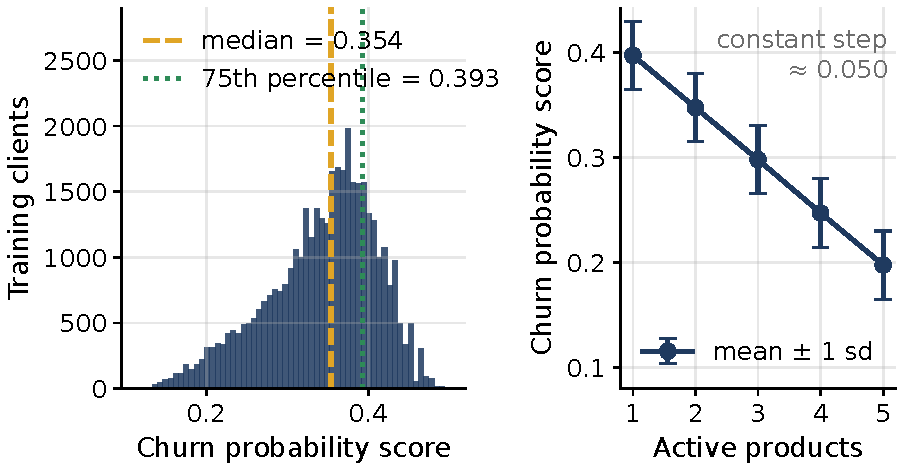
\includegraphics[width=\linewidth]{fig_target.pdf}
  \caption{Izquierda: distribución del puntaje \cp\ en el entrenamiento, con la mediana y el percentil 75 (umbral del
  riesgo alto). Derecha: media y desviación del puntaje por número de productos activos; el paso constante, de unos
  $0{,}050$, delata la regla con la que se generó el puntaje y justifica excluir esa variable.}
  \label{fig:objetivo}
\end{figure}

\subsection{Pipeline y control de fugas}\label{sec:pipeline}

La Figura~\ref{fig:pipeline} resume el pipeline. La partición va antes que todo lo demás: $80/20$ por índices con
semilla $42$ ($n = 38.978$ clientes de entrenamiento y $n_{\mathrm{te}} = 9.745$ de prueba), aleatoria y no por
posición porque el archivo está ordenado por cohortes. La evidencia para eliminar columnas, el umbral $\tau$ y la
fecha de corte de la recencia salen solo de los clientes de entrenamiento, y la prueba no se toca hasta la evaluación
final. El preprocesamiento (imputación, estandarización de las numéricas y booleanas y codificación de las categóricas
con indicadoras) vive dentro de la tubería de cada modelo, de modo que se ajusta solo con las filas de entrenamiento de
cada pliegue.

\begin{figure}[tbp]
  \centering
  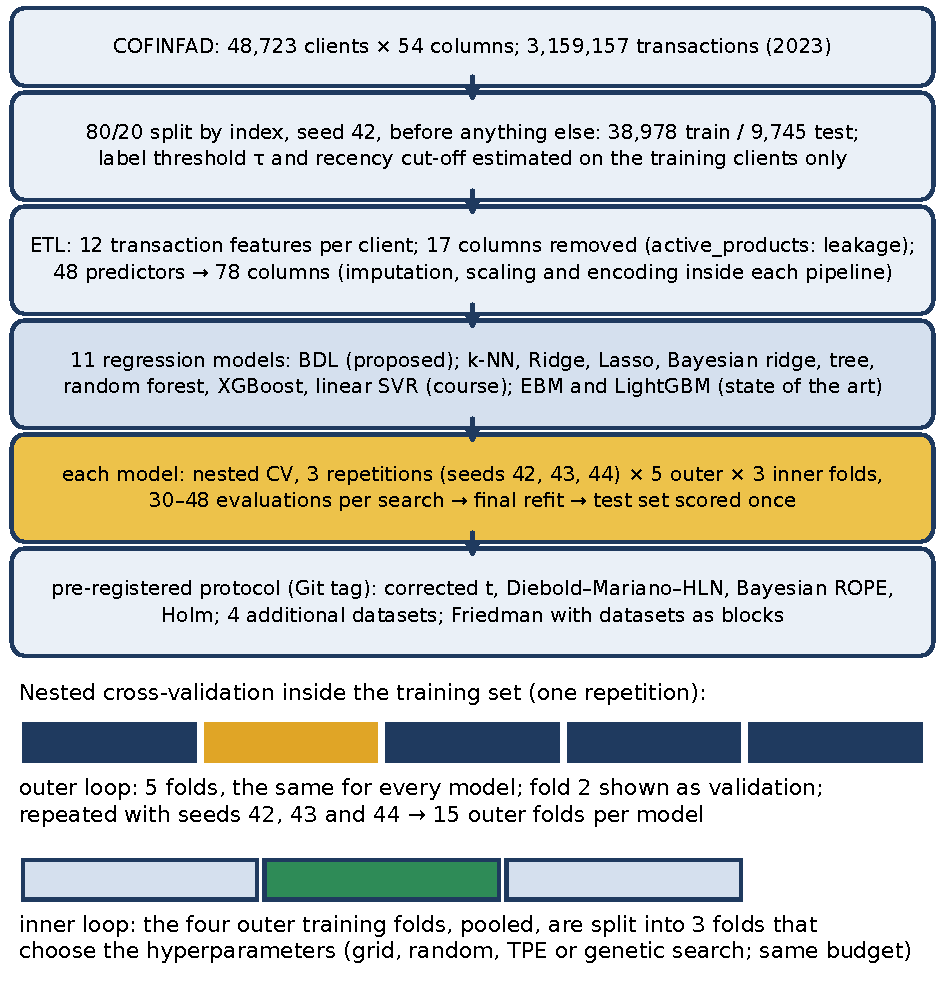
\includegraphics[width=\linewidth]{fig_pipeline.pdf}
  \caption{Pipeline del proyecto final y validación cruzada anidada de cada modelo. La partición se hace primero; el
  bucle externo produce la métrica que se reporta y el interno elige los hiperparámetros; el modelo final se reajusta
  con todo el entrenamiento y toca la prueba una sola vez.}
  \label{fig:pipeline}
\end{figure}

La recencia de un cliente es $\text{corte} - u$, con $u$ la fecha de su última transacción. Antes, la fecha de corte
se tomaba de todo el detalle, que incluye a los clientes de prueba; ahora sale solo del entrenamiento. La corrección
no cambia ningún dato (la fecha es la misma, el 29 de diciembre de 2023) y, además, no podía cambiar un resultado,
porque todos los modelos estandarizan la recencia con la media y la desviación del entrenamiento:
\begin{equation}
  z = \frac{(\text{corte} - u) - (\text{corte} - \bar u)}{s_u} = -\frac{u - \bar u}{s_u},
  \label{eq:recencia}
\end{equation}
que no contiene la fecha de corte. La auditoría de fugas \citep{kapoor2023} comprobó, además, que ningún cliente está
en las dos particiones, que el umbral se estima solo con el entrenamiento y que ningún modelo recibe \ap.

\subsection{Modelos de referencia}\label{sec:referencias}

El modelo propuesto se compara con todos los modelos de regresión del curso: $k$ vecinos más cercanos, Ridge, Lasso,
regresión bayesiana \citep{mackay1992}, árbol de decisión CART, Random Forest \citep{breiman2001}, XGBoost
\citep{chen2016xgboost} y SVR, en su versión lineal porque la de kernel RBF no escala a $38.978$ filas. Se añaden dos
métodos del estado del arte: la EBM \citep{nori2019interpretml} y LightGBM \citep{ke2017}. Todos usan las mismas
particiones, el mismo preprocesamiento y un presupuesto comparable: tantas evaluaciones de hiperparámetros como puntos
tiene la rejilla del modelo (de $30$ a $48$). Para cada benchmark se usa el mejor de cuatro optimizadores (rejilla,
búsqueda aleatoria, TPE de Optuna \citep{akiba2019} y un algoritmo genético), elegido en la entrega anterior; para BDL y
LightGBM, el protocolo fijó TPE. La regresión bayesiana no tiene búsqueda: estima las precisiones del ruido y de los
pesos por máxima evidencia en cada ajuste. La Tabla~\ref{tab:hiperparametros} da el espacio de búsqueda y los
hiperparámetros finales de cada modelo.

\begin{table}[tbp]
  \centering\scriptsize\setlength{\tabcolsep}{3pt}
  \caption{Espacios de búsqueda e hiperparámetros finales de cada modelo de regresión: optimizador elegido con su presupuesto (evaluaciones por búsqueda) y valores que fijó la búsqueda sobre todo el entrenamiento (repetición de la semilla 42).}
  \label{tab:hiperparametros}
  \begin{tabular}{>{\raggedright\arraybackslash}p{0.13\linewidth} >{\raggedright\arraybackslash}p{0.09\linewidth} >{\raggedright\arraybackslash}p{0.38\linewidth} >{\raggedright\arraybackslash}p{0.32\linewidth}}
    \toprule
    Modelo & Búsqueda & Espacio de búsqueda & Hiperparámetros finales \\
    \midrule
    BDL (propuesto) & TPE (30) & $\nu \in [0{,}05;\,1]$ (log); $d \in [1, 6]$; mín. por hoja $\in [5, 200]$ (log); $\lambda \in [0{,}01;\,10]$ (log); bins $M \in [32, 1024]$ (log); $K \in \{$BIC$, 1\}$ & $\nu$ = $0{,}5816$; $d$ = 1; mín. hoja = 88; $\lambda$ = $0{,}0151$; $M$ = 885; $K$ = BIC \\
    XGBoost & TPE (32) & árboles $\in [100, 1000]$ (log); profundidad $\in [2, 10]$; tasa $\in [10^{-3};\,0{,}3]$ (log); submuestreo de filas y de columnas $\in [0{,}5;\,1]$; $\lambda \in [0{,}01;\,10]$ (log); peso mín. por hoja $\in [1, 50]$ (log) & árboles = 512; prof. = 2; tasa = $0{,}0236$; filas = $0{,}80$; columnas = $0{,}73$; $\lambda$ = $0{,}216$; peso mín. = 31 \\
    LightGBM & TPE (32) & árboles $\in [100, 1000]$ (log); hojas $\in [4, 127]$ (log); tasa $\in [10^{-3};\,0{,}3]$ (log); submuestreo de filas y de columnas $\in [0{,}5;\,1]$; $\lambda \in [0{,}01;\,10]$ (log); mín. por hoja $\in [5, 200]$ (log) & árboles = 260; hojas = 4; tasa = $0{,}0508$; filas = $0{,}76$; columnas = $0{,}54$; $\lambda$ = $1{,}686$; mín. hoja = 104 \\
    EBM & rejilla (36) & tasa $\in [0{,}008;\,0{,}1]$ (log); hojas $\in \{2, 3, 4\}$; mín. por hoja $\in [2, 200]$ (log); interacciones $\in [0, 20]$; bins $\in [64, 1024]$ (log) & interacciones = 0; tasa = $8{,}0 \times 10^{-3}$; hojas = 3; mín. hoja = 20; bolsas = 8 \\
    Random Forest & rejilla (36) & profundidad $\in [4, 40]$; variables por corte $\in \{\sqrt{p}, \log_2 p, 0{,}3, 0{,}5\}$; mín. por hoja $\in [1, 100]$ (log); 100 árboles en la búsqueda y 300 en el final & prof. = 8; variables = $0{,}50$; mín. hoja = 50; árboles = 300 \\
    Árbol de decisión & genética (48) & profundidad $\in [3, 30]$; mín. por hoja $\in [1, 300]$ (log); poda $\alpha_{\mathrm{ccp}} \in [10^{-8}, 10^{-4}]$ (log) & prof. = 13; mín. hoja = 101; $\alpha_{\mathrm{ccp}}$ = $1{,}8 \times 10^{-6}$ \\
    Ridge & genética (30) & $\alpha \in [10^{-3}, 10^{5}]$ (log) & $\alpha$ = $613{,}9$ \\
    Lasso & genética (30) & $\alpha \in [10^{-6}, 10^{-1}]$ (log) & $\alpha$ = $1{,}1 \times 10^{-4}$ \\
    Regresión bayesiana & -- & sin búsqueda: las precisiones del ruido y de los pesos se estiman por máxima evidencia en cada ajuste & $\hat\alpha = 262{,}2$; $\hat\lambda = 76.586$ (precisiones estimadas) \\
    SVR lineal & TPE (30) & $C \in [10^{-3}, 10^{2}]$ (log); $\varepsilon \in [10^{-4};\,0{,}05]$ (log) & $C$ = $46{,}43$; $\varepsilon$ = $3{,}8 \times 10^{-4}$ \\
    k-NN & rejilla (32) & $k \in [5, 600]$ (entero, log); pesos uniformes o por distancia; métrica $L_q$, $q \in \{1, 2\}$ & $k$ = 80; $q$ = 1; pesos = distancia \\
    \bottomrule
  \end{tabular}
  \par\smallskip\begin{minipage}{0.97\linewidth}\scriptsize (log): búsqueda en escala logarítmica. El presupuesto es el número de puntos de la rejilla del modelo y se aplica igual con los cuatro optimizadores (rejilla, aleatoria, TPE y genética); el optimizador de cada benchmark es el mejor de los cuatro en el Entregable 3, y el de BDL y LightGBM quedó fijado en el protocolo. En BDL, $\nu$ es la tasa de aprendizaje, $d$ la profundidad de los árboles, $\lambda$ la penalización L2 de las hojas, $M$ el número máximo de intervalos por variable y $K$ el número de clases latentes (BIC: elegido por el criterio BIC; con $K=1$ no hay mezcla).\end{minipage}
\end{table}


\subsection{Modelo propuesto: \emph{boosting} con desplazamiento latente (BDL)}\label{sec:modelo}

\paragraph{Formulación.}
Para un cliente con predictores $\bm{x}$ y puntaje $s$, BDL supone
\begin{equation}
  s = F(\bm{x}) + c_{z} + e, \qquad z \in \{1, \dots, K\}, \quad P(z = k) = \pi_k, \quad e \sim \mathcal{N}(0, \sigma^2),
  \label{eq:modelo}
\end{equation}
con $z$ independiente de $\bm{x}$ y de $e$. $F(\bm{x}) = \beta_0 + \nu \sum_{t=1}^{T} h_t(\bm{x})$ es una suma de árboles
de regresión de profundidad $d$ sobre las variables discretizadas en a lo sumo $M$ intervalos; con $d = 1$ es un modelo
aditivo, con una curva por variable. $z$ es la clase latente, $c_k$ el desplazamiento de la clase $k$, $\pi_k$ su peso y
$\sigma$ la dispersión dentro de cada clase. Con $K = 1$, BDL es el \emph{boosting} de mínimos cuadrados de
\citet{friedman2001}. La log-verosimilitud de $n$ clientes es
\begin{equation}
  \ell(F, \theta) = \sum_{i=1}^{n} \log \sum_{k=1}^{K} \pi_k\, \varphi_\sigma\big(s_i - F(\bm{x}_i) - c_k\big),
  \qquad \theta = (\pi, c, \sigma),
  \label{eq:vero}
\end{equation}
con $\varphi_\sigma$ la densidad normal de media $0$ y desviación $\sigma$. Los supuestos son tres: el desplazamiento es
aditivo y no depende de $\bm{x}$, la clase es independiente de los predictores y la dispersión es la misma en todas las
clases. En COFINFAD se cumplen (sección~\ref{sec:datos}); cuando no, el BIC elige $K = 1$ y BDL se reduce a un
\emph{boosting} de mínimos cuadrados.

\paragraph{Regla de aprendizaje: EM generalizado con paso de \emph{boosting}.}
Maximizar \eqref{eq:vero} directamente es difícil por la suma dentro del logaritmo; el algoritmo EM \citep{dempster1977}
la sustituye por una cota que sí se puede maximizar. Sea $r_i = s_i - F(\bm{x}_i)$ el residuo. El \textbf{paso E}
calcula la probabilidad de que el cliente $i$ pertenezca a la clase $k$:
\begin{equation}
  \gamma_{ik} = \frac{\pi_k\, \varphi_\sigma(r_i - c_k)}{\sum_{l} \pi_l\, \varphi_\sigma(r_i - c_l)}.
  \label{eq:paso-e}
\end{equation}
La esperanza de la log-verosimilitud completa es
$Q(F, \theta) = \sum_i \sum_k \gamma_{ik} \big[\log \pi_k - \log \sigma - (s_i - c_k - F(\bm{x}_i))^2/(2\sigma^2)\big]$
más una constante. Como $\sum_k \gamma_{ik} = 1$, el término cuadrático se separa en
$(\tilde{s}_i - F(\bm{x}_i))^2$ más una varianza que no depende de $F$, con
\begin{equation}
  \tilde{s}_i = s_i - \sum_{k} \gamma_{ik}\, c_k,
  \label{eq:sin-escalon}
\end{equation}
el \textbf{objetivo sin escalón}: el puntaje menos el desplazamiento esperado de su clase. Maximizar $Q$ en $F$ es, por
tanto, minimizar $\sum_i (\tilde{s}_i - F(\bm{x}_i))^2$, y en lugar de resolverlo del todo se dan $B$ pasos de
\emph{boosting}: cada uno ajusta un árbol $h$ al residuo $\tilde{s}_i - F(\bm{x}_i)$ y actualiza $F \leftarrow F + \nu h$.
Cada nodo del árbol elige la variable y el corte que maximizan la ganancia
\begin{equation}
  \frac{G_L^2}{N_L + \lambda} + \frac{G_R^2}{N_R + \lambda} - \frac{G^2}{N + \lambda},
  \qquad v = \frac{G}{N + \lambda},
  \label{eq:ganancia}
\end{equation}
donde $G$ y $N$ son la suma de residuos y el número de filas del nodo, $L$ y $R$ sus hijos y $v$ el valor de una hoja.
El \textbf{paso M} actualiza la mezcla con el índice ya actualizado:
\begin{equation}
  \pi_k = \frac{1}{n}\sum_i \gamma_{ik}, \qquad
  c_k = \frac{\sum_i \gamma_{ik}\, r_i}{\sum_i \gamma_{ik}}, \qquad
  \sigma^2 = \frac{1}{n}\sum_i \sum_k \gamma_{ik}\, (r_i - c_k)^2.
  \label{eq:paso-m}
\end{equation}
El Algoritmo~\ref{alg:bdl} reúne los pasos. El número de clases se elige con el BIC \citep{schwarz1978} sobre el
residuo del calentamiento, con una regla de parsimonia: solo cuentan las clases separadas por al menos $4\sigma$ y con
al menos el $1$~\% de las filas.

\begin{algorithm}[tbp]
  \caption{Ajuste de BDL.}
  \label{alg:bdl}
  \small
  \begin{algorithmic}[1]
    \Require datos $(\bm{x}_i, s_i)_{i=1}^{n}$; tasa $\nu$; profundidad $d$; intervalos $M$; mínimo por hoja; $\lambda$;
             vueltas $V = 400$; árboles por vuelta $B = 5$; calentamiento $T_0 = 100$; $K_{\max} = 8$; paciencia $P = 20$
    \Ensure índice $F$, mezcla $(\pi, c, \sigma)$ y residuos de calibración
    \State Repartir las filas al azar: ajuste ($80$~\%), validación ($10$~\%) y calibración ($10$~\%)
    \State Discretizar cada variable en a lo sumo $M$ intervalos con las filas de ajuste
    \State \textbf{Calentamiento} ($K = 1$): $F \gets \bar{s}$; sumar hasta $T_0$ árboles ajustados a $s_i - F(\bm{x}_i)$, con parada temprana en validación
    \State \textbf{Mezcla inicial}: para $K = 1, \dots, K_{\max}$, $K$-medias exacto en una dimensión sobre los residuos y EM de la mezcla; elegir $K$ por BIC con la regla de parsimonia
    \For{$v = 1, \dots, V$}
      \State \textbf{Paso E}: $\gamma_{ik}$ con \eqref{eq:paso-e} y $\tilde{s}_i$ con \eqref{eq:sin-escalon}
      \State \textbf{Boosting}: $B$ veces, ajustar un árbol $h$ a $\tilde{s}_i - F(\bm{x}_i)$ con \eqref{eq:ganancia} y hacer $F \gets F + \nu h$
      \State \textbf{Paso M}: $\pi$, $c$ y $\sigma$ con \eqref{eq:paso-m}
      \If{el error dentro de clase en validación no mejora en $P$ vueltas} \textbf{parar} \EndIf
    \EndFor
    \State Conservar los árboles y la mezcla de la mejor vuelta y guardar los residuos de calibración
  \end{algorithmic}
\end{algorithm}

\paragraph{Regla de salida.}
En regresión, la predicción es la media del modelo, $\hat{s}(\bm{x}) = F(\bm{x}) + \sum_k \pi_k c_k$. Con los residuos de
calibración se construyen conjuntos de predicción conformes \citep{vovk2005} que usan la densidad de la mezcla como
medida de conformidad: con escalones, cada conjunto es una unión de intervalos cortos, uno por nivel. En clasificación,
la probabilidad de riesgo alto sale del propio modelo como una probabilidad de excedencia:
\begin{equation}
  P(s > \tau \mid \bm{x}) = \sum_{k=1}^{K} \pi_k\, \Phi\!\left(\frac{F(\bm{x}) + c_k - \tau}{\sigma_r}\right),
  \label{eq:excedencia}
\end{equation}
con $\sigma_r$ la dispersión robusta del error dentro de clase medida en validación.

\paragraph{Sustento teórico.}
\emph{La verosimilitud no decrece}: si $\nu \in (0, 2)$ y $\lambda \ge 0$, cada vuelta del Algoritmo~\ref{alg:bdl}
cumple $\ell(F', \theta') \ge \ell(F, \theta)$, y con $\sigma \ge \sigma_{\min} > 0$ la sucesión converge. La razón es
que, por la descomposición de EM, $\ell(F', \theta') - \ell(F, \theta) \ge Q(F', \theta') - Q(F, \theta)$, y ningún paso
baja $Q$: un árbol con hojas de valor $v_l = S_l/(n_l + \lambda)$ cambia la suma de cuadrados en a lo sumo
$-\nu(2 - \nu)\sum_l S_l^2/(n_l + \lambda) \le 0$, y \eqref{eq:paso-m} es el máximo de $Q$ en $\theta$. Además, si las
filas de calibración y un cliente nuevo son intercambiables, los conjuntos de predicción tienen cobertura de al menos
$1 - \alpha$ sin suponer que el modelo sea correcto \citep{vovk2005}. Cada propiedad tiene una prueba unitaria que la
verifica numéricamente.

\paragraph{Implementación.}
\begin{sloppypar}
BDL está programado desde cero con \texttt{numpy} y \texttt{scipy}, en el archivo \texttt{original\_\allowbreak model.py}
del repositorio: la discretización, los árboles por histogramas, el EM de la mezcla, el BIC y la salida conforme. De
scikit-learn solo usa las clases base que dan la interfaz de ajuste y predicción, y la validación de las entradas; una
prueba automática falla si el módulo importa cualquier otra cosa. Las $23$ pruebas unitarias corren en integración continua.
\end{sloppypar}

\subsection{Protocolo de evaluación}\label{sec:protocolo}

\paragraph{Validación.}
Cada modelo se evalúa con validación cruzada anidada \citep{cawley2010}: tres repeticiones (semillas $42$, $43$ y $44$)
de un bucle externo de cinco pliegues, los mismos para todos los modelos, que producen $15$ métricas por modelo; dentro
de cada pliegue externo, un bucle interno de tres pliegues elige los hiperparámetros. El modelo final se reajusta con
todo el entrenamiento y se evalúa una sola vez en la prueba, con un intervalo \emph{bootstrap} BCa \citep{efron1987}.
Las métricas son el RMSE (principal), el MAE, el MAPE y el $R^2$.

\paragraph{Protocolo registrado.}
Antes de los experimentos definitivos se congeló un protocolo con una etiqueta de Git. Sus hipótesis confirmatorias
son que el RMSE de BDL es menor que el del mejor benchmark (H1) y que su AUC es mayor (H2). Fija cuatro pruebas por
benchmark, con Holm \citep{holm1979}: Wilcoxon de rangos con signo y la $t$ corregida sobre los $15$ pliegues, y una
permutación pareada y un \emph{bootstrap} pareado BCa sobre la prueba. BDL se declara superior si su media es mejor
que la del mejor benchmark, al menos tres de las cuatro pruebas rechazan, el efecto no es despreciable ($|\delta| \ge
0{,}147$ o $|d| \ge 0{,}2$) y, en los conjuntos adicionales, es mejor en al menos dos de cuatro y no es
significativamente peor en ninguno.

\paragraph{Pruebas de la guía de resultados.}
Para cumplir la combinación mínima que pide la guía para regresión tabular se añadieron, después del protocolo, la
$t$ corregida de \citet{nadeau2003}, Diebold-Mariano con la corrección de Harvey-Leybourne-Newbold
\citep{diebold1995,harvey1997} y la $t$ correlacionada bayesiana con región de equivalencia práctica de $\pm 0{,}0005$ en
RMSE \citep{benavoli2017}, cada una con Holm sobre las diez referencias; tamaños de efecto ($d$ de Cohen y $A_{12}$);
el \emph{Model Confidence Set} al $90$~\% \citep{hansen2011mcs}, y Friedman con la corrección de Iman-Davenport y
Nemenyi \citep{demsar2006} con los cinco conjuntos de datos como bloques, no los pliegues de uno solo.

\paragraph{Conjuntos adicionales y techo.}
Cuatro conjuntos públicos con objetivo continuo, elegidos antes de conocer el desempeño de ningún modelo: dos con una
variable categórica que desplaza el objetivo retirada a propósito (Seguros médicos y Eficiencia energética), la
situación para la que se diseñó BDL, y dos sin modificar como control (Abulón y Vivienda de California). En cada uno
se usan cinco pliegues externos con la semilla $42$. Como el puntaje se generó a partir de \ap, se calcula además el
techo que deja su exclusión: el error del predictor óptimo que conoce la fórmula del puntaje salvo esa variable.

\paragraph{Ablación.}
La variante registrada retira la mezcla ($K = 1$) y conserva todo lo demás; se compara con las mismas pruebas. Como
análisis exploratorios, se fija $K$ entre $1$ y $8$, se repite la comparación con fracciones del entrenamiento y se
mide la sensibilidad a cada hiperparámetro, a la semilla y al ruido.

\paragraph{Disponibilidad.}
El código, los resultados, el libro del proyecto y el dashboard están en
\url{https://github.com/RubenEsg/Prediccion-de-fuga-de-clientes-en-fintech}, archivado en Zenodo
(\href{https://doi.org/10.5281/zenodo.24356311}{10.5281/zenodo.24356311}); \texttt{generar.py} reproduce cada tabla,
prueba y figura de este informe.

% Sección de resultados del proyecto final (modelo original BDL). Toda cifra sale de datos/ (generar.py).
\section{Resultados}\label{sec:resultados}

Esta sección compara el modelo original del proyecto, BDL (\emph{Boosting} con Desplazamiento Latente), con los modelos
del curso y con dos del estado del arte. Cada cifra sale de \texttt{generar.py}, que reproduce todas las tablas,
pruebas y figuras desde los resultados versionados del proyecto.

\subsection{Resumen del montaje experimental}\label{sec:res-montaje}

Los datos son los $48.723$ clientes sintéticos de COFINFAD \citep{munoz2025}, divididos al azar en
$38.978$ de entrenamiento y $9.745$ de prueba antes de mirar el objetivo; cuatro conjuntos públicos sirven de
contraste. La tarea principal es la regresión del puntaje continuo \cp; la métrica primaria es el RMSE y las
secundarias, MAE, MAPE y $R^2$. Todos los modelos usan el mismo preprocesamiento, las mismas particiones y $30$
evaluaciones de hiperparámetros en una validación anidada: tres repeticiones (semillas $42$, $43$ y $44$) de cinco
pliegues externos ($15$ particiones). El protocolo se registró en Git antes de los experimentos definitivos. Las referencias son $k$-NN, Ridge, Lasso, regresión bayesiana \citep{mackay1992}, árbol de decisión,
Random Forest, XGBoost \citep{chen2016xgboost}, SVR, EBM \citep{nori2019interpretml} y LightGBM \citep{ke2017}. La
regresión bayesiana se añadió después del protocolo, con los mismos pliegues; el SVR es lineal, porque el de kernel
RBF no escala a $38.978$ filas.

\subsection{Desempeño predictivo global}

Las Tablas~\ref{tab:desempeno} y~\ref{tab:prueba} resumen el desempeño en validación cruzada y en prueba. BDL obtiene
el mejor valor en todas las métricas de las dos: RMSE de $0{,}05887 \pm 0{,}00047$ en los pliegues, frente a
$0{,}05897 \pm 0{,}00047$ de XGBoost, el mejor benchmark, y $0{,}05912$ en prueba, frente a $0{,}05917$. Tiene menor
RMSE que cada una de las diez referencias en las $15$ particiones.

\begin{table}[tbp]
  \centering\scriptsize\setlength{\tabcolsep}{4pt}
  \caption{Desempeño en validación cruzada: media $\pm$ desviación en las 15 particiones externas (tres repeticiones de cinco pliegues), en orden de RMSE.}
  \label{tab:desempeno}
  \begin{tabular}{lcccc}
    \toprule
    Modelo & RMSE & MAE & $R^2$ & BDL gana en \\
    \midrule
    BDL (propuesto) & {\boldmath\textbf{$0{,}05887$ $\pm$ $0{,}00047$}} & {\boldmath\textbf{$0{,}04684$ $\pm$ $0{,}00034$}} & {\boldmath\textbf{$0{,}2303$ $\pm$ $0{,}0078$}} & -- \\
    XGBoost$^\dagger$ & \underline{$0{,}05897$ $\pm$ $0{,}00047$} & \underline{$0{,}04689$ $\pm$ $0{,}00032$} & \underline{$0{,}2277$ $\pm$ $0{,}0075$} & 15/15 \\
    LightGBM$^\dagger$ & $0{,}05899$ $\pm$ $0{,}00048$ & $0{,}04693$ $\pm$ $0{,}00034$ & $0{,}2271$ $\pm$ $0{,}0077$ & 15/15 \\
    EBM$^\dagger$ & $0{,}05903$ $\pm$ $0{,}00047$ & $0{,}04704$ $\pm$ $0{,}00033$ & $0{,}2262$ $\pm$ $0{,}0073$ & 15/15 \\
    Random Forest$^\dagger$ & $0{,}05913$ $\pm$ $0{,}00049$ & $0{,}04714$ $\pm$ $0{,}00035$ & $0{,}2234$ $\pm$ $0{,}0078$ & 15/15 \\
    Árbol de decisión$^\dagger$ & $0{,}05928$ $\pm$ $0{,}00048$ & $0{,}04741$ $\pm$ $0{,}00036$ & $0{,}2196$ $\pm$ $0{,}0081$ & 15/15 \\
    Lasso$^\dagger$ & $0{,}06181$ $\pm$ $0{,}00053$ & $0{,}05080$ $\pm$ $0{,}00035$ & $0{,}1515$ $\pm$ $0{,}0084$ & 15/15 \\
    Ridge$^\dagger$ & $0{,}06183$ $\pm$ $0{,}00053$ & $0{,}05076$ $\pm$ $0{,}00035$ & $0{,}1511$ $\pm$ $0{,}0085$ & 15/15 \\
    Regresión bayesiana$^\dagger$ & $0{,}06183$ $\pm$ $0{,}00053$ & $0{,}05075$ $\pm$ $0{,}00035$ & $0{,}1510$ $\pm$ $0{,}0086$ & 15/15 \\
    SVR lineal$^\dagger$ & $0{,}06185$ $\pm$ $0{,}00052$ & $0{,}05086$ $\pm$ $0{,}00033$ & $0{,}1505$ $\pm$ $0{,}0088$ & 15/15 \\
    k-NN$^\dagger$ & $0{,}06334$ $\pm$ $0{,}00052$ & $0{,}05129$ $\pm$ $0{,}00034$ & $0{,}1090$ $\pm$ $0{,}0044$ & 15/15 \\
    \bottomrule
  \end{tabular}
  \par\smallskip\begin{minipage}{0.97\linewidth}\scriptsize En negrita, el mejor de cada columna; subrayado, el segundo. $^\dagger$: la $t$ corregida de Nadeau-Bengio rechaza la igualdad con BDL ($p$ de Holm $<0{,}05$ sobre diez comparaciones). La última columna cuenta las particiones en que BDL tiene menor RMSE. La regresión bayesiana se añadió después del protocolo, con los mismos pliegues: Ridge, reajustado en ellos con sus hiperparámetros guardados, reproduce su RMSE de cada pliegue con una diferencia de $10^{-17}$; sus hiperparámetros se estiman por máxima evidencia.\end{minipage}
\end{table}


\begin{table}[tbp]
  \centering\scriptsize\setlength{\tabcolsep}{6pt}
  \caption{Desempeño en los 9.745 clientes de prueba, con el intervalo bootstrap BCa del 95~\% del RMSE (2000 réplicas).}
  \label{tab:prueba}
  \begin{tabular}{lccccc}
    \toprule
    Modelo & RMSE & IC 95~\% del RMSE & MAE & MAPE (\%) & $R^2$ \\
    \midrule
    BDL (propuesto) & {\boldmath\textbf{$0{,}05912$}} & [$0{,}05831$; $0{,}05992$] & {\boldmath\textbf{$0{,}04697$}} & {\boldmath\textbf{$15{,}96$}} & {\boldmath\textbf{$0{,}2197$}} \\
    XGBoost & \underline{$0{,}05917$} & [$0{,}05836$; $0{,}05996$] & \underline{$0{,}04706$} & \underline{$15{,}98$} & \underline{$0{,}2182$} \\
    LightGBM & $0{,}05918$ & [$0{,}05838$; $0{,}05997$] & $0{,}04707$ & \underline{$15{,}98$} & $0{,}2181$ \\
    EBM$^\ddagger$ & $0{,}05925$ & [$0{,}05845$; $0{,}06006$] & $0{,}04720$ & $16{,}03$ & $0{,}2161$ \\
    Random Forest$^\ddagger$ & $0{,}05931$ & [$0{,}05851$; $0{,}06011$] & $0{,}04728$ & $16{,}05$ & $0{,}2146$ \\
    Árbol de decisión$^\ddagger$ & $0{,}05944$ & [$0{,}05863$; $0{,}06025$] & $0{,}04750$ & $16{,}11$ & $0{,}2112$ \\
    Lasso$^\ddagger$ & $0{,}06166$ & [$0{,}06086$; $0{,}06251$] & $0{,}05072$ & $17{,}10$ & $0{,}1511$ \\
    Ridge$^\ddagger$ & $0{,}06167$ & [$0{,}06087$; $0{,}06253$] & $0{,}05069$ & $17{,}10$ & $0{,}1509$ \\
    Regresión bayesiana$^\ddagger$ & $0{,}06167$ & [$0{,}06088$; $0{,}06253$] & $0{,}05069$ & $17{,}10$ & $0{,}1508$ \\
    SVR lineal$^\ddagger$ & $0{,}06170$ & [$0{,}06091$; $0{,}06256$] & $0{,}05073$ & $17{,}10$ & $0{,}1499$ \\
    k-NN$^\ddagger$ & $0{,}06321$ & [$0{,}06234$; $0{,}06405$] & $0{,}05115$ & $17{,}28$ & $0{,}1080$ \\
    \bottomrule
  \end{tabular}
  \par\smallskip\begin{minipage}{0.97\linewidth}\scriptsize En negrita, el mejor de cada columna; subrayado, el segundo. $^\ddagger$: Diebold-Mariano-HLN sobre el error cuadrático de cada cliente rechaza la igualdad con BDL ($p$ de Holm $<0{,}05$). El MAPE solo se calcula en prueba, porque el protocolo no guardó los pronósticos de cada pliegue.\end{minipage}
\end{table}


La mejora absoluta sobre XGBoost es de $0{,}000099$ en los pliegues ($0{,}17$~\%) y de $0{,}000058$ en prueba
($0{,}10$~\%). Frente a los modelos lineales es de unos $0{,}0030$ ($4{,}8$~\%) y frente a $k$-NN, de $0{,}0045$
($7{,}1$~\%). La Figura~\ref{fig:folds} muestra dos grupos separados: los seis modelos de árboles, entre $0{,}0589$ y
$0{,}0593$, y los lineales y $k$-NN, por encima de $0{,}0618$. Dentro del primer grupo, las cajas se solapan casi por
completo y los intervalos BCa del RMSE en prueba \citep{efron1987} también.

\begin{figure}[tbp]
  \centering
  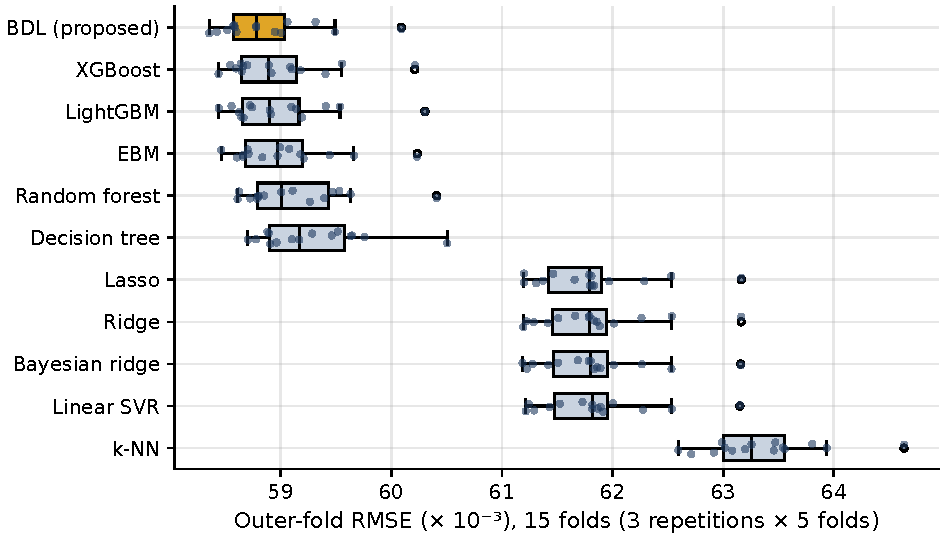
\includegraphics[width=\linewidth]{fig_folds}
  \caption{RMSE de cada modelo en las 15 particiones externas (tres repeticiones de cinco pliegues). Cada punto es una
  partición; BDL, en ámbar, tiene la mediana más baja. Los modelos de árboles forman un grupo y los lineales y $k$-NN,
  otro, unos $0{,}003$ más arriba.}
  \label{fig:folds}
\end{figure}

La ventaja no puede ser mucho mayor. El predictor óptimo, que conoce la fórmula del puntaje salvo la variable
excluida \ap, obtiene $0{,}05911$ en prueba y $0{,}05887$ en los pliegues: BDL queda a $0{,}00001$ en prueba y a
$0{,}000007$ en los pliegues de ese techo, y XGBoost, a $0{,}00007$ en prueba. El $R^2$ ronda $0{,}22$ porque la parte
del puntaje que depende de \ap{} no se puede predecir con los predictores disponibles.

La Figura~\ref{fig:regression} muestra esa estructura. El puntaje observado frente al pronosticado forma cinco bandas
paralelas, una por nivel de \ap. Los residuos de BDL se concentran en cinco picos estrechos separados por $0{,}05$:
el modelo separa casi por completo la señal observable del escalón latente. Los de XGBoost forman los mismos picos,
pero más anchos.

\begin{figure}[tbp]
  \centering
  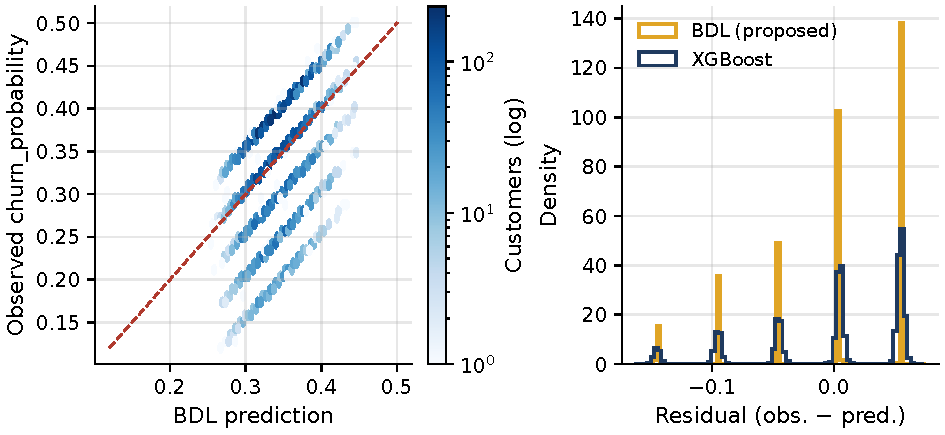
\includegraphics[width=\linewidth]{fig_regression}
  \caption{Izquierda: puntaje observado frente al pronóstico de BDL en los 9.745 clientes de prueba (escala logarítmica
  de conteos); la línea discontinua es la identidad. Las cinco bandas corresponden a los cinco niveles de la variable
  excluida \texttt{active\_products}. Derecha: densidad de los residuos de BDL y de XGBoost.}
  \label{fig:regression}
\end{figure}

\subsection{Resultados de las pruebas de significancia}

Se aplicó la combinación mínima que la guía exige para regresión tabular: la $t$ corregida de \citet{nadeau2003} sobre
las $15$ particiones, Diebold-Mariano \citep{diebold1995} con la corrección de \citet{harvey1997} sobre el error
cuadrático de cada cliente de prueba y la $t$ correlacionada bayesiana con región de equivalencia práctica (ROPE)
\citep{corani2015,benavoli2017}. Cada prueba se ajustó con Holm \citep{holm1979} sobre las diez referencias, con
$\alpha=0{,}05$. La ROPE es de $\pm0{,}0005$ en RMSE (cerca del $0{,}85$~\%), la misma de la versión anterior de esta
sección, fijada antes de calcular. Acompañan a cada $p$ la diferencia con su intervalo del $95$~\%, la $d$ de Cohen
\citep{cohen1988} y la $A_{12}$ de \citet{vargha2000}. La Tabla~\ref{tab:pruebas} y la Figura~\ref{fig:intervals}
reúnen los resultados.

\begin{table}[tbp]
  \centering\scriptsize\setlength{\tabcolsep}{1.8pt}
  \caption{Pruebas de significancia de BDL frente a cada referencia (combinación mínima de la guía para regresión tabular). $\Delta$: RMSE de la referencia menos RMSE de BDL, $\times 10^{3}$ (positivo: BDL se equivoca menos).}
  \label{tab:pruebas}
  \begin{tabular}{lcccccccc}
    \toprule
    Referencia & $\Delta$ pliegues [IC 95~\%] & $t$ corr. & $p_{\mathrm{Holm}}$ & DM-HLN & $p_{\mathrm{Holm}}$ & P(mejor / ROPE / peor) & $d$ & $A_{12}$ \\
    \midrule
    XGBoost & $+0{,}099$ [$0{,}053$; $0{,}144$] & $4{,}62$ & $0{,}001$ & $2{,}00$ & $0{,}092$ & $0{,}00$ / $1{,}00$ / $0{,}00$ & $0{,}21$ & $0{,}60$ \\
    LightGBM & $+0{,}119$ [$0{,}051$; $0{,}186$] & $3{,}77$ & $0{,}003$ & $1{,}92$ & $0{,}092$ & $0{,}00$ / $1{,}00$ / $0{,}00$ & $0{,}25$ & $0{,}60$ \\
    EBM & $+0{,}153$ [$0{,}068$; $0{,}239$] & $3{,}86$ & $0{,}003$ & $2{,}81$ & $0{,}015$ & $0{,}00$ / $1{,}00$ / $0{,}00$ & $0{,}33$ & $0{,}64$ \\
    Random Forest & $+0{,}260$ [$0{,}155$; $0{,}366$] & $5{,}30$ & $4{,}5 \times 10^{-4}$ & $3{,}51$ & $0{,}002$ & $0{,}00$ / $1{,}00$ / $0{,}00$ & $0{,}54$ & $0{,}72$ \\
    Árbol de decisión & $+0{,}407$ [$0{,}260$; $0{,}554$] & $5{,}93$ & $1{,}8 \times 10^{-4}$ & $4{,}78$ & $8{,}9 \times 10^{-6}$ & $0{,}10$ / $0{,}90$ / $0{,}00$ & $0{,}86$ & $0{,}76$ \\
    Lasso & $+2{,}939$ [$2{,}660$; $3{,}219$] & $22{,}55$ & $1{,}9 \times 10^{-11}$ & $13{,}70$ & $1{,}5 \times 10^{-41}$ & $1{,}00$ / $0{,}00$ / $0{,}00$ & $5{,}88$ & $1{,}00$ \\
    Ridge & $+2{,}954$ [$2{,}672$; $3{,}235$] & $22{,}50$ & $1{,}9 \times 10^{-11}$ & $13{,}75$ & $9{,}4 \times 10^{-42}$ & $1{,}00$ / $0{,}00$ / $0{,}00$ & $5{,}93$ & $1{,}00$ \\
    Regresión bayesiana & $+2{,}956$ [$2{,}672$; $3{,}240$] & $22{,}32$ & $1{,}9 \times 10^{-11}$ & $13{,}76$ & $9{,}1 \times 10^{-42}$ & $1{,}00$ / $0{,}00$ / $0{,}00$ & $5{,}94$ & $1{,}00$ \\
    SVR lineal & $+2{,}973$ [$2{,}682$; $3{,}265$] & $21{,}87$ & $1{,}9 \times 10^{-11}$ & $13{,}85$ & $3{,}0 \times 10^{-42}$ & $1{,}00$ / $0{,}00$ / $0{,}00$ & $6{,}03$ & $1{,}00$ \\
    k-NN & $+4{,}470$ [$4{,}174$; $4{,}767$] & $32{,}33$ & $1{,}5 \times 10^{-13}$ & $17{,}38$ & $1{,}2 \times 10^{-65}$ & $1{,}00$ / $0{,}00$ / $0{,}00$ & $9{,}02$ & $1{,}00$ \\
    \bottomrule
  \end{tabular}
  \par\smallskip\begin{minipage}{0.97\linewidth}\scriptsize $t$ corregida de Nadeau-Bengio sobre las 15 particiones (14 grados de libertad, intervalo con la misma varianza corregida); Diebold-Mariano con la corrección de Harvey-Leybourne-Newbold sobre el error cuadrático de los 9.745 clientes de prueba; $p$ ajustados con Holm sobre las diez referencias en cada prueba ($\alpha=0{,}05$). Prueba bayesiana: $t$ correlacionada con ROPE de $\pm0{,}0005$ en RMSE; probabilidades posteriores de que BDL sea mejor, equivalente o peor. $d$ de Cohen y $A_{12}$ de Vargha-Delaney entre los valores por pliegue (positivo y mayor que $0{,}5$ favorecen a BDL). BDL tiene menor RMSE que cada referencia en las 15 particiones.\end{minipage}
\end{table}


La $t$ corregida rechaza la igualdad frente a las diez referencias. Frente a XGBoost, la diferencia media es de
$0{,}099 \times 10^{-3}$, con intervalo $[0{,}053;\ 0{,}144] \times 10^{-3}$, $t=4{,}62$ y $p_{\mathrm{Holm}}=0{,}001$.
Diebold-Mariano rechaza frente a ocho: no lo hace frente a XGBoost ($p_{\mathrm{Holm}}=0{,}092$) ni frente a LightGBM
($0{,}092$). En prueba, la ventaja sobre XGBoost es de $0{,}058 \times 10^{-3}$ y su intervalo BCa,
$[0{,}005;\ 0{,}117] \times 10^{-3}$, apenas excluye el cero. En resumen, \textbf{BDL supera significativamente a ocho
de las diez referencias con las dos pruebas frecuentistas} ($p_{\mathrm{Holm}}<0{,}05$) y, frente a XGBoost y
LightGBM, solo con la $t$ corregida.

\begin{figure}[tbp]
  \centering
  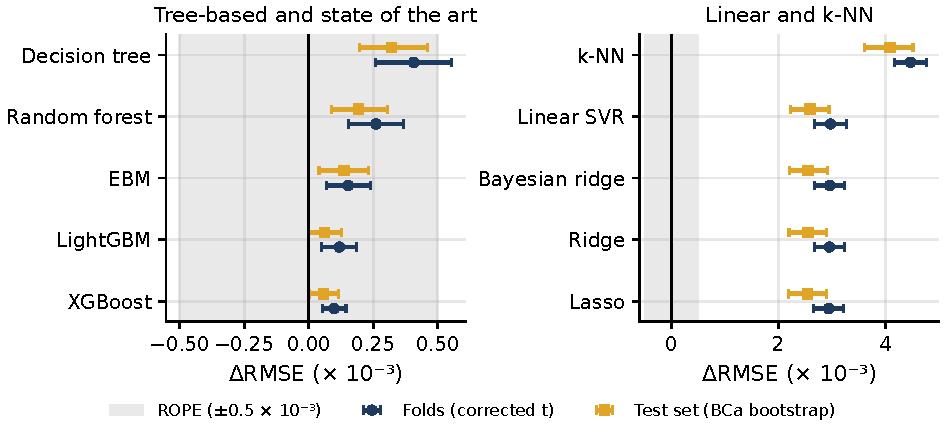
\includegraphics[width=\linewidth]{fig_intervals}
  \caption{Diferencia de RMSE de cada referencia menos BDL ($\times 10^{-3}$; positiva: BDL se equivoca menos), con
  su intervalo del 95~\%: en las 15 particiones (varianza corregida de Nadeau-Bengio, azul) y en los 9.745 clientes de
  prueba (bootstrap BCa, ámbar). La franja gris es la región de equivalencia práctica ($\pm 0{,}5 \times 10^{-3}$).
  A la izquierda, los modelos de árboles; a la derecha, los lineales y $k$-NN, en otra escala.}
  \label{fig:intervals}
\end{figure}

La prueba bayesiana distingue la significancia estadística de la relevancia práctica. BDL es mejor con probabilidad
posterior $1{,}000$ que los cuatro lineales y $k$-NN. Frente a XGBoost, LightGBM, EBM y Random Forest, la probabilidad
de que la diferencia caiga en la ROPE es de al menos $0{,}9999$: \textbf{BDL es prácticamente equivalente a esos
cuatro}. Frente al árbol, la posterior se reparte entre equivalencia ($0{,}903$) y superioridad ($0{,}097$). Las
diferencias frente a los modelos de árboles, de $0{,}10$ a $0{,}41 \times 10^{-3}$, equivalen a entre el $20$~\% y el
$81$~\% de la ROPE.

Los tamaños de efecto coinciden con esa lectura: $d=0{,}21$ y $A_{12}=0{,}60$ frente a XGBoost; $d=0{,}86$ y
$A_{12}=0{,}76$ frente al árbol; $d$ cercana a $6$ y $A_{12}=1$ frente a los lineales.

Las pruebas discrepan frente a XGBoost y LightGBM por la potencia, no por un error. La $t$ corregida usa $15$
métricas por pliegue y BDL gana en todas. Diebold-Mariano usa un solo conjunto de prueba, en el que la varianza del
error de cada cliente, dominada por el escalón latente, es enorme frente a una diferencia de RMSE de $0{,}000058$.
Wilcoxon de rangos con signo \citep{wilcoxon1945}, como verificación, rechaza frente a las diez
($p_{\mathrm{Holm}}=0{,}0006$), aunque comparte la dependencia entre pliegues. El \emph{Model Confidence Set}
\citep{hansen2011mcs} al $90$~\% sobre las pérdidas de prueba solo retiene a BDL; XGBoost y LightGBM salen con
$p=0{,}098$, justo en el borde.

El veredicto confirmatorio sigue siendo el del protocolo registrado, cuyas cuatro pruebas incluían dos en prueba:
frente a XGBoost rechazan Wilcoxon y la $t$ corregida, pero no la permutación pareada ($p_{\mathrm{Holm}}=0{,}092$) ni
el bootstrap BCa ($0{,}076$). Dos de cuatro no alcanzan las tres que exige la condición de superioridad, así que BDL
no se declara superior.

\begin{table}[tbp]
  \centering\scriptsize\setlength{\tabcolsep}{3pt}
  \caption{BDL en los cuatro conjuntos adicionales: RMSE medio en los cinco pliegues externos (semilla 42) del mejor benchmark de cada conjunto y de BDL, ventaja relativa (positiva si BDL es mejor), $p$ de la $t$ corregida y puesto entre los modelos.}
  \label{tab:conjuntos}
  \begin{tabular}{llccccc}
    \toprule
    Conjunto & Mejor benchmark & RMSE benchmark & RMSE BDL & Ventaja & $p$ ($t$ corr.) & Puesto \\
    \midrule
    Seguros médicos & EBM & $11.332$ & $11.435$ & $-0{,}90$~\% & $0{,}414$ & 8 de 11 \\
    Eficiencia energética & EBM & $2{,}2634$ & $2{,}3128$ & $-2{,}18$~\% & $0{,}474$ & 2 de 11 \\
    Abulón & Random Forest & $2{,}1293$ & $2{,}1683$ & $-1{,}83$~\% & $0{,}286$ & 5 de 11 \\
    Vivienda de California & LightGBM & $0{,}4426$ & $0{,}4645$ & $-4{,}95$~\% & $0{,}002$ & 3 de 11 \\
    \bottomrule
  \end{tabular}
  \par\smallskip\begin{minipage}{0.97\linewidth}\scriptsize Friedman con los 5 conjuntos como bloques y 11 modelos: $\chi^2=22{,}58$, $p=0{,}012$; Iman-Davenport $p=0{,}003$. Rango medio de BDL: $3{,}8$; diferencia crítica de Nemenyi: $6{,}75$ (Figura~\ref{fig:cd}).\end{minipage}
\end{table}


La Tabla~\ref{tab:conjuntos} y la Figura~\ref{fig:cd} amplían la comparación a cinco conjuntos. Friedman con la
corrección de Iman-Davenport \citep{demsar2006,iman1980} detecta diferencias entre los $11$ modelos ($\chi^2=22{,}58$,
$p=0{,}012$), pero la diferencia crítica de Nemenyi, $6{,}75$ rangos, no separa a ningún par de modelos. Los cinco
primeros son EBM ($2{,}8$), XGBoost ($3{,}4$), BDL ($3{,}8$), LightGBM ($4{,}0$) y Random Forest ($4{,}8$). BDL no es
mejor que el mejor benchmark en ninguno de los cuatro conjuntos adicionales, y es significativamente peor en Vivienda
de California ($-4{,}95$~\%, $p=0{,}002$). Con cinco conjuntos la potencia de Friedman es baja; la guía recomienda
diez o más.

\begin{figure}[tbp]
  \centering
  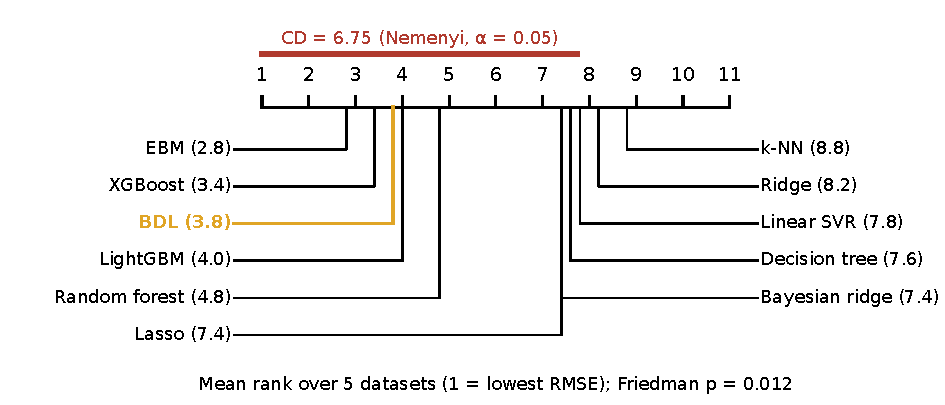
\includegraphics[width=\linewidth]{fig_cd}
  \caption{Diagrama de diferencia crítica con los cinco conjuntos de datos (COFINFAD y los cuatro adicionales) como
  bloques: rango medio de cada modelo por RMSE (1 = el mejor). Los modelos cuyos rangos difieren menos que la barra
  roja (Nemenyi, $\alpha=0{,}05$) no se distinguen; BDL, en ámbar, no se distingue de ninguno.}
  \label{fig:cd}
\end{figure}

\subsection{Resultados del estudio de ablación}

El componente propio de BDL es la mezcla latente de desplazamientos. La hipótesis registrada era que retirarla
($K=1$, un \emph{boosting} de mínimos cuadrados con los mismos árboles) aumenta el RMSE. La Tabla~\ref{tab:ablacion} y
la Figura~\ref{fig:ablation} aplican las mismas pruebas de la comparación principal.

\begin{table}[tbp]
  \centering\scriptsize\setlength{\tabcolsep}{1.8pt}
  \caption{Ablación de la mezcla latente en regresión: RMSE en los cinco pliegues externos de la semilla 42 y en prueba. Aporte: RMSE de la variante menos RMSE de BDL completo, $\times 10^{3}$ (positivo: la mezcla ayuda).}
  \label{tab:ablacion}
  \begin{tabular}{lccccccc}
    \toprule
    Variante & RMSE (pliegues) & Aporte [IC 95~\%] & $p$ ($t$ corr.) & P(ROPE) & RMSE prueba & Aporte prueba & $p$ (DM) \\
    \midrule
    BDL completo & $0{,}05887$ $\pm$ $0{,}00041$ & -- & -- & -- & $0{,}05912$ & -- & -- \\
    Sin mezcla ($K=1$) & $0{,}05898$ $\pm$ $0{,}00041$ & $+0{,}107$ [$0{,}008$; $0{,}205$] & $0{,}040$ & $0{,}9998$ & $0{,}05910$ & $-0{,}016$ & $0{,}623$ \\
    \midrule
    $K=1$ fijo & $0{,}05902$ $\pm$ $0{,}00040$ & $+0{,}142$ & -- & -- & -- & -- & -- \\
    $K=2$ fijo & $0{,}05897$ $\pm$ $0{,}00041$ & $+0{,}085$ & -- & -- & -- & -- & -- \\
    $K=3$ fijo & $0{,}05894$ $\pm$ $0{,}00039$ & $+0{,}053$ & -- & -- & -- & -- & -- \\
    $K=4$ fijo & $0{,}05889$ $\pm$ $0{,}00041$ & $+0{,}013$ & -- & -- & -- & -- & -- \\
    $K=5$ fijo & $0{,}05888$ $\pm$ $0{,}00041$ & $0{,}000$ & -- & -- & -- & -- & -- \\
    $K=6$ fijo & $0{,}05888$ $\pm$ $0{,}00041$ & $0{,}000$ & -- & -- & -- & -- & -- \\
    $K=8$ fijo & $0{,}05888$ $\pm$ $0{,}00041$ & $0{,}000$ & -- & -- & -- & -- & -- \\
    $K$ por BIC (final) & $0{,}05888$ $\pm$ $0{,}00041$ & -- & -- & -- & -- & -- & -- \\
    \bottomrule
  \end{tabular}
  \par\smallskip\begin{minipage}{0.97\linewidth}\scriptsize Las dos primeras filas son la ablación registrada, con las mismas pruebas de la comparación principal (hiperparámetros elegidos por la búsqueda en cada pliegue). Las demás vienen del análisis de sensibilidad: la configuración final con $K$ fijo o elegido por BIC, en los mismos pliegues y sin nueva búsqueda; son exploratorias y su aporte se mide frente a la última fila (positivo: la variante es peor).\end{minipage}
\end{table}


En los cinco pliegues de la semilla $42$, retirar la mezcla aumenta el RMSE en $0{,}107 \times 10^{-3}$, con
intervalo $[0{,}008;\ 0{,}205] \times 10^{-3}$, en los cinco pliegues y con $p=0{,}040$ en la $t$ corregida: la
hipótesis se confirma en validación cruzada. En prueba no se confirma: la variante sin mezcla queda
$0{,}016 \times 10^{-3}$ por delante ($p=0{,}62$ en Diebold-Mariano). La prueba bayesiana pone el aporte dentro de la
ROPE con probabilidad $0{,}9998$: con todos los datos, la mezcla mejora poco en la práctica.

Dos análisis exploratorios explican de dónde sale el aporte. Al fijar $K$, el RMSE baja con cada clase hasta cinco:
$+0{,}142$, $+0{,}085$, $+0{,}053$ y $+0{,}013 \times 10^{-3}$ para $K$ de $1$ a $4$, y $0$ desde $K=5$. El criterio
BIC elige $K=5$, el número real de niveles de \ap. Además, la ganancia de la mezcla crece cuando hay pocos datos:
$0{,}748 \times 10^{-3}$ ($1{,}3$~\%) con $3.118$ filas, $0{,}337$ con $7.796$, $0{,}187$ con $15.591$ y $0{,}142$
con $31.182$. Al restar del objetivo el escalón esperado, el \emph{boosting} aprende el índice con menos ruido, y eso
pesa más cuando hay pocas filas.

\begin{figure}[tbp]
  \centering
  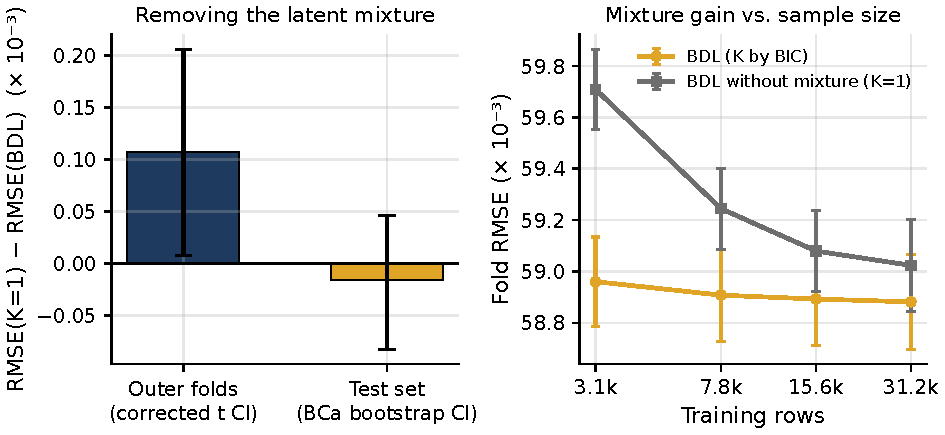
\includegraphics[width=\linewidth]{fig_ablation}
  \caption{Izquierda: aporte de la mezcla latente, RMSE sin mezcla ($K=1$) menos RMSE de BDL ($\times 10^{-3}$), con su
  intervalo del 95~\% en los cinco pliegues de la semilla 42 ($t$ corregida) y en prueba (bootstrap BCa). Derecha: RMSE
  por pliegue de BDL con y sin mezcla según el número de filas de entrenamiento (media $\pm$ error estándar en cinco
  pliegues).}
  \label{fig:ablation}
\end{figure}

\subsection{Sensibilidad y robustez}

La variación entre semillas es despreciable frente a las diferencias entre modelos (Tabla~\ref{tab:semillas}). Al
reajustar el modelo final con diez semillas, la desviación del RMSE en prueba es de $1{,}7 \times 10^{-6}$ en BDL,
frente a $5{,}0 \times 10^{-6}$ en XGBoost y $12{,}3 \times 10^{-6}$ en LightGBM. El orden de los modelos no depende de
la semilla.

\begin{table}[tbp]
  \centering\scriptsize\setlength{\tabcolsep}{3pt}
  \caption{Variación entre semillas del modelo final: RMSE en prueba al reajustar con diez semillas.}
  \label{tab:semillas}
  \begin{tabular}{lccc}
    \toprule
    Modelo & RMSE medio & Desviación ($\times 10^{-6}$) & Semillas \\
    \midrule
    BDL (propuesto) & $0{,}059116$ & $1{,}7$ & 10 \\
    XGBoost & $0{,}059171$ & $5{,}0$ & 10 \\
    LightGBM & $0{,}059183$ & $12{,}3$ & 10 \\
    EBM & $0{,}059259$ & $6{,}8$ & 10 \\
    Random Forest & $0{,}059306$ & $10{,}4$ & 10 \\
    \bottomrule
  \end{tabular}
\end{table}


La Figura~\ref{fig:sensitivity} resume las otras dos pruebas. A la derecha, al cambiar un hiperparámetro a la vez en
los mismos pliegues, $30$ de $34$ configuraciones quedan por delante de XGBoost con sus hiperparámetros finales
($0{,}05896$). Solo la tasa de aprendizaje de $0{,}05$ pierde más de una desviación entre pliegues ($0{,}05959$). A la
izquierda, la curva de aprendizaje: BDL con $3.118$ filas ($0{,}05896$) iguala a XGBoost con $31.182$.

Ante datos contaminados, BDL es el mejor de los tres \emph{boostings} en $8$ de $11$ escenarios. Pierde con ruido
gaussiano fuerte en el objetivo (desviación de $0{,}02$ o más) y con ruido fuerte en los predictores numéricos: la
mezcla supone escalones nítidos, y el ruido los desdibuja.

\begin{figure}[tbp]
  \centering
  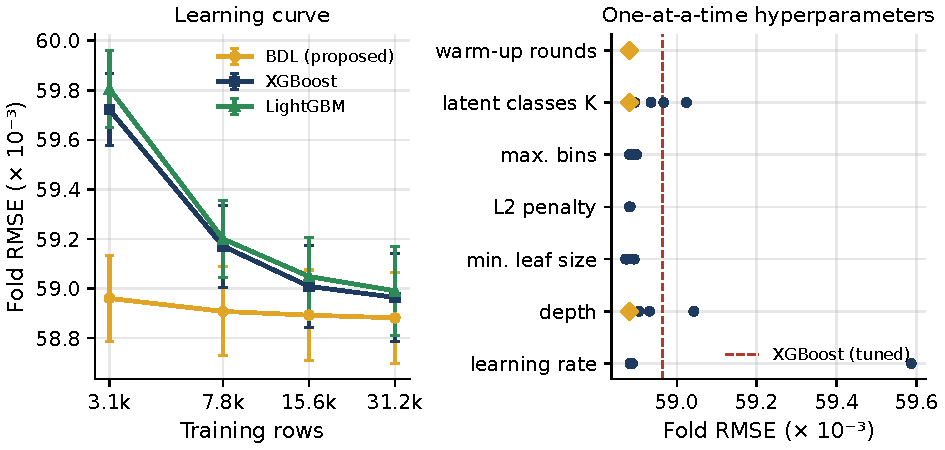
\includegraphics[width=\linewidth]{fig_sensitivity}
  \caption{Izquierda: curva de aprendizaje, RMSE por pliegue (media $\pm$ error estándar en cinco pliegues de la
  semilla 42) según las filas de entrenamiento, para BDL, XGBoost y LightGBM. Derecha: sensibilidad a cada
  hiperparámetro de BDL, cambiando uno a la vez respecto de la configuración final (rombo ámbar); la línea discontinua
  es XGBoost con sus hiperparámetros finales en los mismos pliegues.}
  \label{fig:sensitivity}
\end{figure}

\subsection{Costo computacional}

La Tabla~\ref{tab:costo} reúne el costo de cada modelo final. BDL tarda $5{,}8$~s en ajustarse con los $38.978$
clientes: $3{,}4$ veces lo de XGBoost ($1{,}7$~s), aunque menos que Random Forest ($11{,}2$~s) y la EBM ($25{,}5$~s).
Predice los $9.745$ clientes de prueba en $0{,}068$~s, unos $7$~$\mu$s por cliente, casi lo mismo que XGBoost. Su
memoria pico ($153$~MB) es la de XGBoost, y guarda $16.420$ parámetros en $149$~KB. En cuanto a si vale la pena: con todos los
datos, la ganancia de $0{,}17$~\% no justifica por sí sola triplicar el tiempo de ajuste. Sí lo justifica cuando los
datos son escasos (Figuras~\ref{fig:ablation} y~\ref{fig:sensitivity}) o cuando importa la estructura del error.

\begin{table}[tbp]
  \centering\scriptsize\setlength{\tabcolsep}{4pt}
  \caption{Costo computacional del modelo final de cada referencia: ajuste con todo el entrenamiento (38.978 clientes) e inferencia sobre los 9.745 de prueba (medias de diez semillas), memoria pico del ajuste, tamaño serializado y número de parámetros.}
  \label{tab:costo}
  \begin{tabular}{lccccc}
    \toprule
    Modelo & Ajuste (s) & Inferencia (s) & Memoria (MB) & Tamaño (KB) & Parámetros \\
    \midrule
    k-NN & $0{,}26$ & $4{,}889$ & $64$ & $6.295$ & 3.079.262 \\
    Regresión bayesiana & $0{,}35$ & $0{,}044$ & -- & $50$ & 79 \\
    Ridge & $0{,}41$ & $0{,}047$ & $67$ & $4$ & 79 \\
    Lasso & $0{,}42$ & $0{,}048$ & $65$ & $4$ & 79 \\
    LightGBM & $0{,}60$ & $0{,}062$ & $66$ & $46$ & 5.436 \\
    SVR lineal & $0{,}65$ & $0{,}048$ & $72$ & $4$ & 79 \\
    Árbol de decisión & $0{,}81$ & $0{,}047$ & $55$ & $6$ & 69 \\
    XGBoost & $1{,}69$ & $0{,}063$ & $154$ & $58$ & 3.899 \\
    BDL (propuesto) & $5{,}80$ & $0{,}068$ & $153$ & $149$ & 16.420 \\
    Random Forest & $11{,}25$ & $0{,}130$ & $66$ & $2.347$ & 86.158 \\
    EBM & $25{,}54$ & $0{,}055$ & $81$ & $1.032$ & 15.486 \\
    \bottomrule
  \end{tabular}
  \par\smallskip\begin{minipage}{0.97\linewidth}\scriptsize Equipo: AMD Ryzen 5 3500X (6 núcleos), 16 GB de RAM, Windows 11, sin GPU; Python 3.13.3. Parámetros: coeficientes en los modelos lineales; nodos en los árboles y conjuntos de árboles; celdas de las funciones de forma en la EBM; en BDL, las celdas de sus 78 funciones de forma (los 2.020 tocones se acumulan en ellas), los cortes y la mezcla; en k-NN, la matriz de entrenamiento que guarda. La memoria de la regresión bayesiana no se midió con el mismo procedimiento.\end{minipage}
\end{table}


\subsection{Interpretabilidad y análisis de errores}

La importancia por permutación en los clientes de prueba \citep{breiman2001} muestra que BDL y XGBoost usan las mismas
tres variables (Figura~\ref{fig:importance}). Barajar \texttt{age} aumenta el RMSE de BDL en $8{,}46 \times 10^{-3}$;
\texttt{app\_\allowbreak logins\_\allowbreak frequency}, en $5{,}56 \times 10^{-3}$, y
\texttt{satisfaction\_\allowbreak score}, en
$2{,}51 \times 10^{-3}$. Ninguna otra variable pasa de $0{,}04 \times 10^{-3}$. Es lo esperable en un conjunto
generado con reglas: el puntaje depende de esas tres variables y de \ap. BDL las aprovecha algo más que XGBoost
($7{,}95$, $5{,}30$ y $1{,}89 \times 10^{-3}$), porque aprende su índice sin el ruido del escalón.

\begin{figure}[tbp]
  \centering
  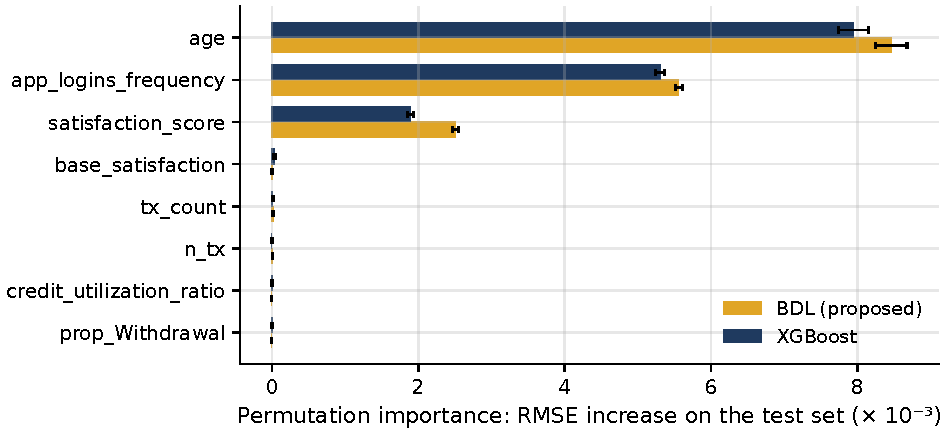
\includegraphics[width=\linewidth]{fig_importance}
  \caption{Importancia por permutación en los 9.745 clientes de prueba: aumento del RMSE al barajar cada variable
  original (media y desviación de cinco repeticiones), para BDL y XGBoost, con sus modelos finales de la semilla 43.
  Se muestran las ocho variables de mayor importancia.}
  \label{fig:importance}
\end{figure}

La mezcla de BDL es interpretable por sí misma. El modelo final tiene cinco clases con pesos $0{,}402$, $0{,}301$,
$0{,}149$, $0{,}098$ y $0{,}050$, separadas por $0{,}050$. Las proporciones reales de \ap{} en entrenamiento son
$0{,}402$, $0{,}301$, $0{,}149$, $0{,}099$ y $0{,}050$, con un escalón de $0{,}05$. \textbf{BDL recuperó la
distribución de la variable excluida sin verla.}

\begin{table}[tbp]
  \centering\scriptsize\setlength{\tabcolsep}{5pt}
  \caption{Error en prueba por subgrupo de clientes y por quintil del objetivo: BDL frente a XGBoost. Diferencia: RMSE de XGBoost menos RMSE de BDL, $\times 10^{3}$ (positiva: BDL se equivoca menos).}
  \label{tab:errores}
  \begin{tabular}{lcccc}
    \toprule
    Subgrupo & Clientes & RMSE BDL & RMSE XGBoost & Diferencia \\
    \midrule
    Todos & 9.745 & $0{,}05912$ & $0{,}05917$ & $+0{,}058$ \\
    \midrule
    Edad 29 & 1.643 & $0{,}05928$ & $0{,}05942$ & $+0{,}134$ \\
    Edad 30 & 1.581 & $0{,}06012$ & $0{,}06010$ & $-0{,}026$ \\
    Edad 44 & 1.598 & $0{,}05843$ & $0{,}05853$ & $+0{,}094$ \\
    Edad 45 & 1.576 & $0{,}05830$ & $0{,}05830$ & $-0{,}005$ \\
    Edad 59 & 1.631 & $0{,}05858$ & $0{,}05869$ & $+0{,}112$ \\
    Edad 60 & 1.716 & $0{,}05989$ & $0{,}05993$ & $+0{,}037$ \\
    \midrule
    \texttt{tx\_count} $>$ 500 (cola) & 134 & $0{,}06306$ & $0{,}06344$ & $+0{,}376$ \\
    \texttt{tx\_count} $\leq$ 500 & 9.611 & $0{,}05906$ & $0{,}05911$ & $+0{,}053$ \\
    \midrule
    Segmento inactive & 1.954 & $0{,}05874$ & $0{,}05875$ & $+0{,}016$ \\
    Segmento occasional & 3.852 & $0{,}05870$ & $0{,}05877$ & $+0{,}069$ \\
    Segmento power & 1.026 & $0{,}05885$ & $0{,}05894$ & $+0{,}085$ \\
    Segmento regular & 2.913 & $0{,}06000$ & $0{,}06006$ & $+0{,}063$ \\
    \midrule
    Quintil 1 del objetivo [$0{,}120$; $0{,}287$] & 1.954 & $0{,}09929$ & $0{,}09951$ & $+0{,}220$ \\
    Quintil 2 del objetivo [$0{,}287$; $0{,}337$] & 1.987 & $0{,}03802$ & $0{,}03722$ & $-0{,}791$ \\
    Quintil 3 del objetivo [$0{,}337$; $0{,}370$] & 1.910 & $0{,}03618$ & $0{,}03511$ & $-1{,}068$ \\
    Quintil 4 del objetivo [$0{,}370$; $0{,}400$] & 1.959 & $0{,}04607$ & $0{,}04567$ & $-0{,}399$ \\
    Quintil 5 del objetivo [$0{,}401$; $0{,}501$] & 1.935 & $0{,}05215$ & $0{,}05369$ & $+1{,}547$ \\
    \bottomrule
  \end{tabular}
\end{table}


El análisis de errores (Tabla~\ref{tab:errores}) señala dónde falla. Por subgrupo, BDL se equivoca menos que XGBoost
en $10$ de $12$, con la mayor ventaja en la cola de clientes con más de $500$ transacciones ($+0{,}376 \times 10^{-3}$).
Por quintil del objetivo, los dos modelos fallan más en los extremos: en el primero sobrestiman el puntaje en
$0{,}091$ y en el último lo subestiman en $0{,}050$. Es la regresión hacia la media que impone el escalón no
observable. BDL es mejor en los dos extremos ($+0{,}22$ y $+1{,}55 \times 10^{-3}$), justo en el de mayor riesgo, y
algo peor en los tres quintiles centrales (entre $-0{,}40$ y $-1{,}07 \times 10^{-3}$).

\subsection{Discusión, limitaciones y amenazas a la validez}

BDL funciona en COFINFAD porque el puntaje tiene la forma que el modelo supone: una función suave de tres variables
más un escalón aditivo que depende de una variable excluida. El \emph{boosting} aprende esa función sobre el objetivo
sin escalón, y por eso BDL queda a $0{,}00001$ del predictor óptimo en prueba. Es lo que se observa en los árboles con
efectos aleatorios \citep{hajjem2014,sigrist2022}: restar del objetivo un efecto de grupo antes de ajustar los árboles
los vuelve más eficientes; BDL lo hace sin observar el grupo. La ventaja es pequeña porque el techo está cerca: XGBoost
ya estaba a $0{,}00007$. En los conjuntos adicionales no hay un desplazamiento aditivo nítido (la búsqueda de
hiperparámetros eligió $K=1$ en los cuatro), y BDL se reduce a un \emph{boosting} programado desde cero, menos refinado
que XGBoost o LightGBM.

En clasificación, la tarea secundaria, BDL obtiene un AUC de $0{,}8313 \pm 0{,}0038$ en los pliegues (quinto de diez),
frente a $0{,}8333 \pm 0{,}0041$ de XGBoost, y ninguna prueba rechaza la igualdad. La superioridad no se cumple en
ninguna de las dos tareas.

Limitaciones. Los datos son sintéticos: las conclusiones no se trasladan a clientes reales. Cinco conjuntos
dan poca potencia a Friedman, y Diebold-Mariano descansa en un solo conjunto de prueba. La ROPE es una decisión del
equipo: con una más estrecha, la equivalencia práctica con los \emph{boostings} podría no sostenerse. La regresión
bayesiana, Diebold-Mariano y la prueba bayesiana se añadieron después del protocolo; son exploratorias y no cambian el
veredicto. Falta el SVR con kernel RBF. La auditoría no detectó fugas de
información.

La evidencia sugiere que BDL es el modelo más preciso en COFINFAD, con una ventaja estadísticamente detectable en
validación cruzada pero prácticamente equivalente a la de los mejores \emph{boostings}, y que esa ventaja no se
generaliza a otros conjuntos.

% Conclusiones del informe del proyecto final (modelo original BDL).
\section{Conclusiones}\label{sec:conclusiones}

El análisis exploratorio mostró que el puntaje de COFINFAD es un índice de pocas variables más un escalón constante que
depende de una variable que hay que excluir. BDL convierte ese hallazgo en un modelo: una suma de árboles más una
mezcla latente de desplazamientos, ajustada con una regla de aprendizaje propia, un EM generalizado cuyo paso M es un
paso de \emph{boosting} contra el objetivo sin escalón, programada desde cero y con la garantía de que la verosimilitud
no decrece.

En COFINFAD, BDL es el modelo más preciso: el menor error en las cuatro métricas, tanto en validación cruzada como en
prueba, y a $0{,}00001$ de RMSE del predictor óptimo. Su ventaja sobre los mejores \emph{boostings} es estadísticamente
detectable en validación cruzada, pero pequeña en la práctica, y no alcanza las tres pruebas que exige el protocolo
para declararlo superior. Tampoco se generaliza: en los cuatro conjuntos adicionales no hay un escalón nítido y BDL no
supera al mejor benchmark de ninguno. En clasificación queda al nivel de los mejores, sin diferencias significativas.

Su valor está en otra parte. Recupera la distribución de la variable excluida sin verla, con cinco clases cuyos pesos
coinciden con las proporciones reales; necesita diez veces menos datos para alcanzar el error de XGBoost, y varía
menos entre semillas que XGBoost, LightGBM, la EBM y Random Forest. La ablación confirma que la mezcla aporta en validación cruzada
y que su aporte crece cuando hay pocos datos.

Las principales limitaciones son que los datos son sintéticos, que cinco conjuntos dan poca potencia a las
comparaciones entre conjuntos y que algunas pruebas se añadieron después del protocolo. Como trabajo futuro quedan
hacer que los pesos de las clases dependan de los predictores, permitir una dispersión distinta por clase y validar el
modelo con datos reales y con fuga observada.


\bibliographystyle{elsarticle-harv}
\bibliography{referencias}

\end{document}
